\documentclass[twocolumn]{article}
\usepackage{graphicx} % Required for inserting images
\usepackage{caption}
\usepackage{amsmath}



\title{Lab 3: Planetary Nebula}
\author{Elaine Ran}
\date{October 3, 2025}

\begin{document}

\maketitle

\section{Introduction}
The ultimate goal of this lab was to reproduce the Hertzsprung-Russell (H-R) diagram using our data collected via the Andor CCD camera at the Hartung-Boothroyd Observatory. Our data comes from M11, an open cluster.

\section{Setup}
For this experiment we are using a high-performance spectroscopic CCD camera (Andor CCD) and a telescope. We first zero the telescope coordinates by finding Vega and setting that as the zero point. Vega has a right ascension (RA) of $18^h36^m56.3^s$ and a declination (Dec) of $-38^{\circ}47^{\prime}01.3^{\prime\prime}$. 

\section{Bias and Dome Flats}
For \textbf{bias} measurements we put the black filter into the camera and took photos with zero exposure time. We must subtract the bias from our data to account for the electronic offset and readout noise introduced by the CCD. For \textbf{dome flats}, we closed the dome, and put in our red, green and blue filters to take images. These dome flats prominently show dust and other contamination on the CCD that we must factor into our science source images. 
\\
\\
To calculate the bias level, we read in data using \verb|astropy.io.fits|. We then create a bias array which is a 2D 512 x 2048 array in which each value \verb|i, j| corresponds to the median of all the bias frames values \verb|i, j|. 
\\
\\
To get flats for each filter, we read in each of the flat frames and divide by the median of that flat frame (to normalize the frame) and add them to an array of the flat frames. Then, we take the median of the array to create a flat array which is a 2D 512 x 2048 array in which each value \verb|i, j| corresponds to the median of all the flat frames values \verb|i, j|. 

\section{Science Source Data}
We move our telescope and camera to M11. The M11 cluster has a RA of $18^h51^m05.0^s$ and a dec of $-06^{\circ}16^{\prime}12.0^{\prime\prime}$. We then took five images for each of the three filters, red, green and blue. An example of an image taken is shown in figure~\ref{fig:redex} 
\begin{figure}[h!]
    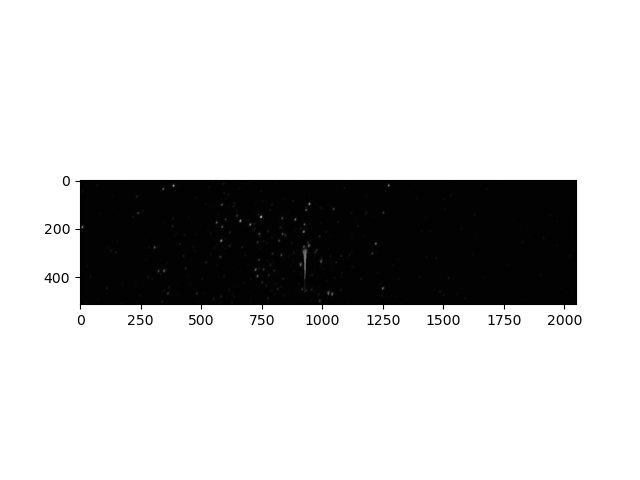
\includegraphics[width=0.5\textwidth]{Figures/redfilterexample.png}
    \caption{Example of a M11 image taken by the Andor CCD with the red filter and 3 second exposure time.}
    \label{fig:redex}
\end{figure}
\\
\\
For the analysis, we subtract the bias array and then divide by the flat array and add it to an array. Then, we take the median of this array to create a science source array which is a 2D 512 x 2048 array in which each value \verb|i, j| corresponds to the median of all the science source frames values \verb|i, j|. 
\\
\\
To detect stars, we use \verb|DAOStarFinder| from \verb|photutils.detection|: 
\\
\\
\\
\begin{verbatim}
    mean, median, std = 
        sigma_clipped_stats(data, sigma=5.0)
    daofind = DAOStarFinder(fwhm=3,
        threshold=5 * std)
    sources = daofind(data - median, 
        mask=mask)
\end{verbatim}
The mask excludes the bright star near the center of the image with bleeding. We can visualize what the \verb|daofind| found by drawing circles around the positions of the detected sources. An example can be seen in figure ~\ref{fig:greenex}.
\begin{verbatim}
    circle_size = 5
    positions = np.transpose(
        (sources['xcentroid'], 
        sources['ycentroid']))
    apertures = CircularAperture(positions, 
        r=circle_size)
\end{verbatim}
\begin{figure}[h!]
    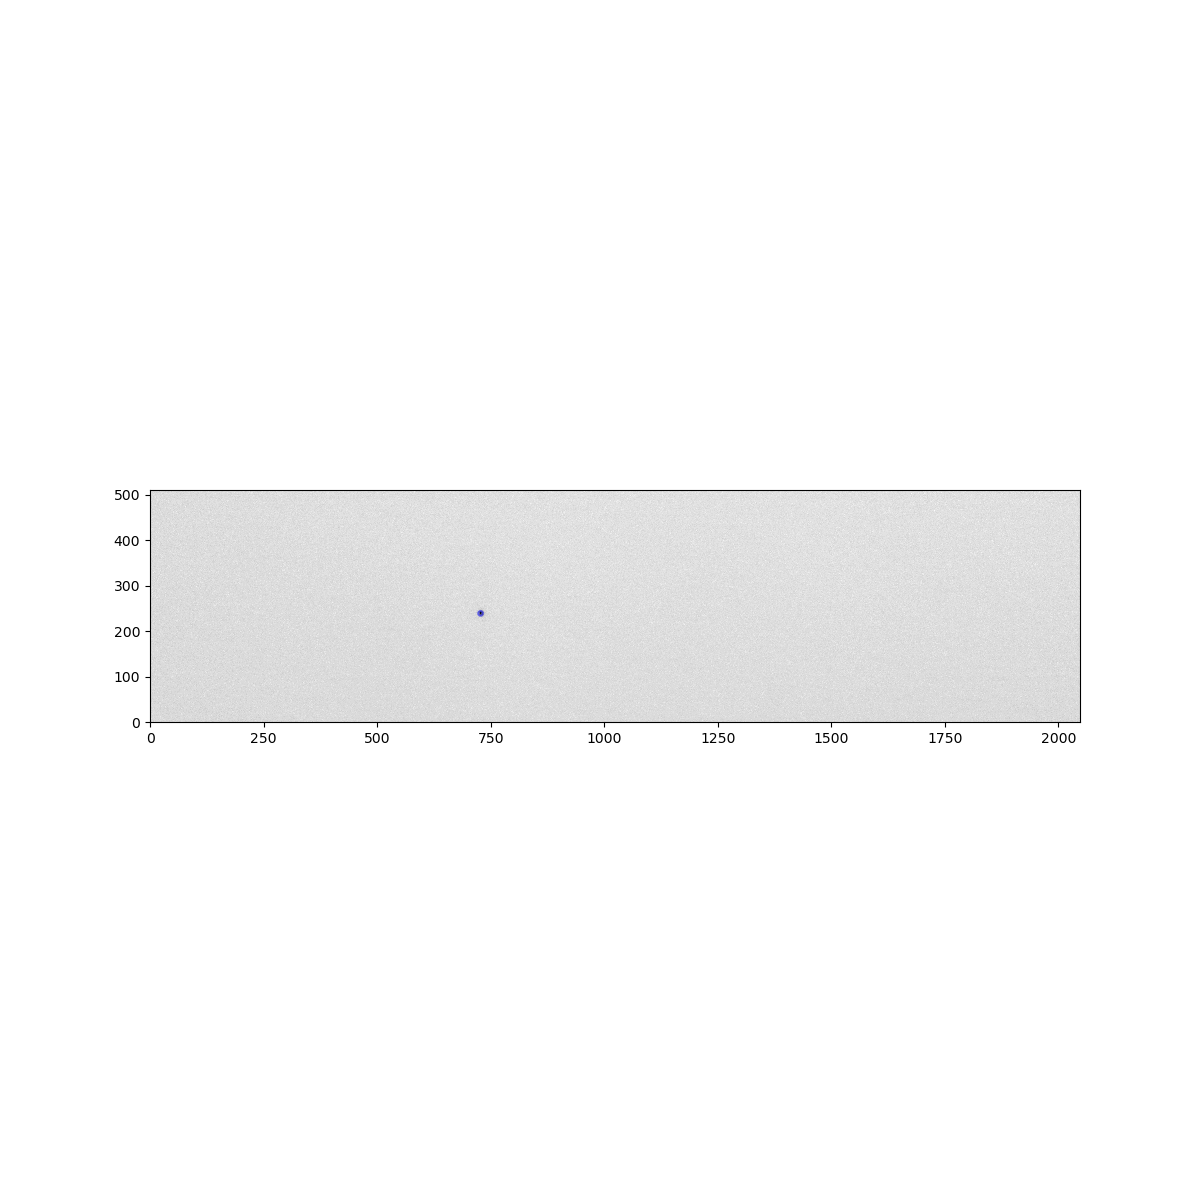
\includegraphics[width=0.5\textwidth]{Figures/examplegreenwithsources.png}
    \caption{Example of a M11 image taken by the Andor CCD with the green filter and 10 second exposure time with detected sources circled in blue.}
    \label{fig:greenex}
\end{figure}
We need to know the brightness of these detected stars. To do this, we must perform aperture photometry on each detected star. This is the process of measuring flux from a star from within a circular aperture, and subtracting the background/sky brightness that is measured in an annulus around the star. We can do this using using the \verb|aperture_photometry| method from \verb|photutils.aperture|:
\begin{verbatim}
    annulus_aperture = CircularAnnulus(positions, 
        r_in=10, r_out=15)
    aperstats = ApertureStats(data, 
        annulus_aperture)
    bkg_mean = aperstats.mean
    aperture_area = apertures.area_overlap(data)
    total_bkg = bkg_mean * aperture_area
    phot_table = aperture_photometry(data, 
        apertures)
    phot_bkgsub = phot_table['aperture_sum'] 
        - total_bkg
    phot_table['total_bkg'] = total_bkg
    phot_table['aperture_sum_bkgsub'] = phot_bkgsub
\end{verbatim}
This gives us a table of the x and y pixel coordinates of the input aperture center(s) and the sum of the values within the aperture in surface brightness units, the total background summed in the annulus and the difference between the values within the aperture and the annulus. An example of the table returned by \verb|aperture_photometry| is in table ~\ref{tab:greenex}.

\begin{table}[h!]
\centering
\begin{tabular}{r r r r r r}
\hline
ID & xcenter & ycenter & aperture\_sum & total\_bkg & aperture\_sum\_bkgsub \\
\hline
 1 &  401.273 &   0.710 & 1393.2105 & 444.6538 &  948.5567 \\
 2 & 1289.312 &   0.598 & 1931.0014 & 259.5625 & 1671.4389 \\
 3 & 1108.651 &   6.932 & 1576.5726 & 350.8818 & 1225.6908 \\
 4 & 1107.228 &   7.487 & 1614.4346 & 347.7176 & 1266.7170 \\
 5 &  360.253 &  11.060 & 3199.1500 & 745.5752 & 2453.5749 \\
 6 &  358.248 &  12.127 & 3265.3018 & 739.0982 & 2526.2036 \\
 7 &  762.716 &  21.036 & 1146.4168 & 386.1002 &  760.3166 \\
 8 &  249.850 &  42.355 & 1287.9529 & 496.1782 &  791.7747 \\
 9 &  896.179 &  60.457 & 2196.3798 & 383.9167 & 1812.4631 \\
10 &  651.467 &  69.362 & 1546.4575 & 622.0544 &  924.4031 \\
\hline
\end{tabular}
\captionsetup{position=bottom}
\caption{Table of 10 of the sources detected by the green filter (with exposure time of 10 seconds) for images taken of M11. }
\label{tab:greenex}
\end{table}
I used the apertures returned by performing aperture photometry on the green/visible filter for the other filters as well. This is because performing aperture photometry on each filter independently leads to a different number of stars detected since some stars are brighter in one filter and faint in another. I chose the green/visible filter as the standard since the red one seemed to have the most stars and the blue one was the faintest, so the green/visible filter seemed to be a good in-between. 

When plotting these apertures from the green filter against the other filters, I noticed there was a slight shift between the positions of the apertures and the stars in these filters. I decided that there must have been some slight shift in the images when the filters were switched out, so I simply adjusted the positions so they fit the stars better. 
\section{Calibration}
To accurately get magnitudes from our science source, we must calibrate it with a standard star, which, in the case of M11 is HD 175544. We move our telescope and camera to HD 175544 which is has a RA of $18^h53^m13.1^s$ and a dec of $00^{\circ}11^{\prime}59.0^{\prime\prime}$. We then took five images of this calibration star for each of the filters. An example can be seen in figure ~\ref{fig:calibblue}.
\begin{figure}[h!]
    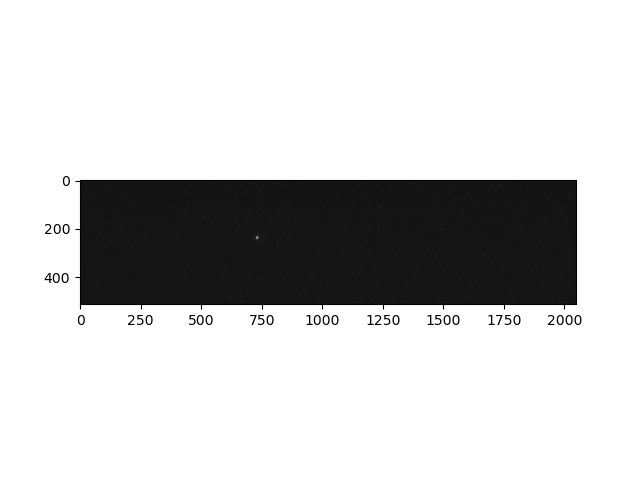
\includegraphics[width=0.5\textwidth]{Figures/calibblue.png}
    \caption{Example of an image of calibration star for M11, HD 175544, taken by the Andor CCD with the blue filter and 0.1 second exposure time.}
    \label{fig:calibblue}
\end{figure}
\subsection{Photometric Zero Point}
We can repeat much of the steps from the science source star detection here to get the brightness of the calibration star in each filter to get a table of sources (which should just be the one calibration star) for the images. Then, to determine the photometric zero point $Z_F$ we use the equation $Z_F = m + 2.5 \log S$ where $m$ is the known magnitude of the calibration star in this filter and $S$ is the signal in $DU/s$. In code (for the green filter) this is:
\begin{verbatim}
    green_zp = 7.395 + 2.5 * 
        np.log10(g_c['aperture_sum_bkgsub']
            / 0.3)
\end{verbatim}
where \verb|g_c| is the table of sources for the calibration star with green filter. 7.395 comes from the handout which states the V value of HD 175544 is 7.395 and 0.3 comes in because we need to get our signal to be in $DN/s$ and thus must divide \verb|g_c['aperture_sum']| by the exposure time (which was 0.3 seconds for the green filter).

Doing this for all three filters we get these values for the photometric zero point: 
\[
\begin{aligned}
Z_{F_{red}} &= 7.321 + 2.5\log(S/0.1) = 19.54 \\
Z_{F_{green}} &= 7.395 + 2.5\log(S/0.3) = 18.57 \\
Z_{F_{blue}} &= 7.502 + 2.5\log(S/0.1) = 18.10
\end{aligned}
\]
\subsection{Image Quality (FWHM)}
To find the image quality in full-width half-maximum (FWHM) we can use the \verb|fit_fwhm| function from \verb|photutils.psf|. The code is:
\begin{verbatim}
    sources = daofind(data - median, 
        mask=mask)
    xypos = list(zip(sources['xcentroid'], 
        sources['ycentroid']))
    fwhm = np.median(fit_fwhm(data - median, 
        xypos=xypos, fit_shape=(5, 5)))
\end{verbatim}
Doing this for all three filters we get these values for image quality in FWHM: 
\[
\begin{aligned}
\mathrm{Red (FWHM)} &= 5.66 \\
\mathrm{Green (FWHM)} &= 7.36 \\
\mathrm{Blue (FWHM)} &= 6.16
\end{aligned}
\]
These are for the images of M11, not the calibration star.
\subsection{Sky Brightness}
For the sky brightness in magnitudes per square arcsecond, we use the photometric zero point calculated before to find the magnitude, and then divide by the area of the pixels. The code is:
\begin{verbatim}
def sky_brightness(median, exp, zp):
    sps = median / exp
    area = (0.325)**2  
    return zp - 2.5 * np.log10(sps / area)
\end{verbatim}
Doing this for all three filters we get these values for sky brightness: 
\[
\begin{aligned}
\mathrm{SB_{Red}} &= 10.45 \mathrm{mag}\,\mathrm{arcsec}^{-2} \\
\mathrm{SB_{Green}} &= 11.63 \mathrm{mag}\,\mathrm{arcsec}^{-2}\\
\mathrm{SB_{Blue}} &= 11.36 \mathrm{mag}\,\mathrm{arcsec}^{-2}
\end{aligned}
\]
\subsection{Airmass}
To get the airmass of the observations, we use the latitude and longitude of Hartung-Boothroyd as well as the right ascension and declination of M11. Doing this for all three filters we get these values for airmass:
\[
\begin{aligned}
\mathrm{Airmass_{Red}} &= 1.537 \\
\mathrm{Airmass_{Green}} &= 1.543\\
\mathrm{Airmass_{Blue}} &= 1.550
\end{aligned}
\]
\section{Color Magnitude Diagrams}
Now that we know the photometric zero points, we can get the magnitudes in the green and blue filters to plot the color magnitude diagram. The equation we need is $m_F = Z_F - 2.5\log S\prime$. 
\begin{verbatim}
B = blue_zp - 2.5*
    np.log10(blue_sources['aperture_sum_bkgsub']/10)
V = green_zp - 2.5*
    np.log10(green_sources['aperture_sum_bkgsub']/10)
\end{verbatim}
For this diagram, I cropped out some outlier values at $B-V > 3$ and $B-V < -0.5$. The diagram is in figure ~\ref{fig:cmd}
\begin{figure}[h!]
    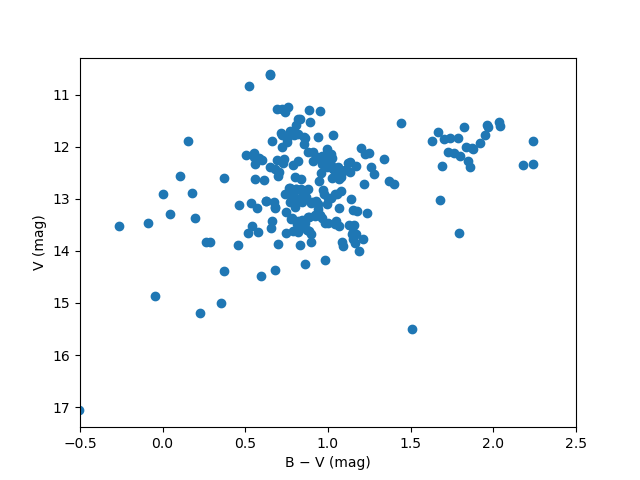
\includegraphics[width=0.5\textwidth]{Figures/CMD.png}
    \caption{Color magnitude diagram of M11 from our data. Y-axis is flipped so that brighter stars are at top/left.}
    \label{fig:cmd}
\end{figure}

\section{Conclusion}
The CMD doesn't look exactly as I would expect. Since M11 is an open cluster, there are a lot of young main sequence stars, so I assumed our CMD would have a clear main sequence with a negative slope in the CMD. However, after looking at some other CMD plots for M11 from the reference paper attatched to the assignment, it seems that my CMD captures the turn-off point for main sequence stars (based on the V and B-V values as well as the overall shape). I tried playing around with changing the radius of the apertures as well as the standard filter for star detection, but the CMD looks relatively similar in every case with similar range of V and B-V as well. One explanation is that B and V are possibly flipped, since the only way I can tell is from lab notes during observation. 















\end{document}
